\section{Motivation}
\label{s:motivation}

% - characteristics of concurrency bugs
% - challenges / design requirements
% - limitations of existing approaches

This work is motivated by an observation that none of previous works
incorporates a coverage metric that properly addresses characteristics
of \textit{offending thread interleaving} (\ie, one that causes a
concurrency bug).
%
As a consequence, previous works either \textbf{1)} may use a
too-simplified coverage metric, and not be able to identify whether
offending thread interleaving remains untested~\cite{krace}, or
\textbf{2)} may waste the computing power by executing too many
redundant instances of thread interleaving~\cite{snowboard, razzer}.


In this section, we first comprehend why concurrency bugs manifest
depending on thread interleaving through a real-world concurrency bug
example.
%
We then define design requirements to effectively discover concurrency
bugs in the kernel, and summarize why existing approaches do not
satisfy the design requirements.


\PP{Manifestation of concurrency bugs}
%
\begin{figure}[t]
  \centering
  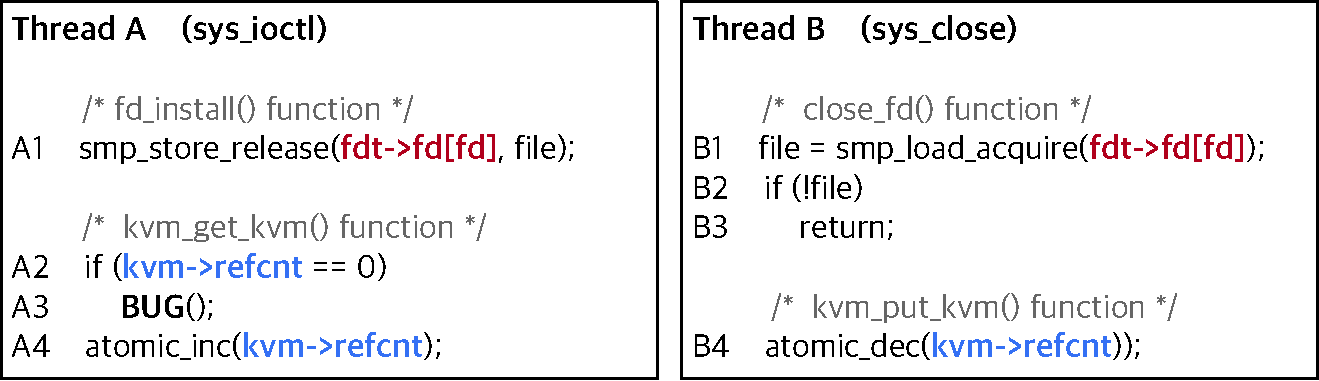
\includegraphics[width=0.95\linewidth]{fig/cve-2017-10661.pdf}
  \caption{Simplified code snippet of CVE-2017-7533. If \texttt{B1} is
    executed between \texttt{A2} and \texttt{A4}, a race condition on
    \texttt{inet->hdrincl} leads to uninitialized stack pointer usage
    on \texttt{rfv}, and an attacker may gain root privileges.}
  \label{fig:cve-2019-6974}
\end{figure}
%
\autoref{fig:cve-2019-6974} describes how an erroneous instance of
thread interleaving causes a concurrency bug.
%
In this example, an uninitialized access bug may manifest when two
system calls are executed concurrently: \texttt{sendmsg()} to send a
message through an ipv4 socket, and \texttt{setsockopt()} to modify an
option of the ipv4 socket. As a consequence of the uninitialized
access bug, an attacker may gain root privileges.



Assuming \texttt{inet->hdrincl} is initially \texttt{1}, the race
condition manifests depending on the execution order of three memory
accesses, \texttt{A2} and \texttt{A4} in thread~A, and \texttt{B1} and
in thread~B.
%
During sending a message through the ipv4 socket, thread~A reads a
value of \texttt{inet->hdrincl} twice at \texttt{A2} and \texttt{A4}.
%
However, since these two read operations are not atomically executed,
thread~B may intervene in the middle of these two read operations.
%
In that case, if \texttt{B1} is executed between \texttt{A2} and
\texttt{A4}, thread~A may read different values of
\texttt{inet->hdrincl} at \texttt{A2} and \texttt{A4}, and dereference
\texttt{rfv} without initializing it.



As can seen in this example, the manifestation of a concurrency bug is
\textit{a combined result of a few scheduling constraints}, where each
scheduling constraint is established on a pair of instructions.
%
In this example, \texttt{rfv} is not initialized only if \texttt{A2}
is executed before \texttt{B1}. Thus, the uninitialized access
requires a scheduling constraint
$\texttt{A1} \rightarrow \texttt{B1}$~\footnote{In this paper,
  $\texttt{X} \rightarrow \texttt{Y}$ denotes that \texttt{X} is
  executed before \texttt{Y}}.
%
Similary, a scheduling constraint on \texttt{B1} and \texttt{A4} also
is required for the concurrency bug to manifest since thread~A
dereferences uninitialized \texttt{rfv} only if
$\texttt{B1} \rightarrow \texttt{A4}$.
%
In summary, among all possible instances of thread interleaving, the
concurrency bug manifests \textit{only if} the two scheduling
constraints are conjunctively satisfied, \ie,
$(\texttt{A1} \rightarrow \texttt{B1}) \wedge (\texttt{B4} \rightarrow
\texttt{A2})$.


\PP{Design requirements}
%
\dr{This part looks too similar with Razzer}
%
The main goal of this paper is to design a fuzzing technique to
effectively discover kernel concurrency bugs. To this end, we elicit
design requirements of a concurrency fuzzer as follows:

\vspace{0.4em}
%
\textbf{R1}: \emph{A fuzzer should be able to determine that offending
  thread interleaving remains untested.}

\textbf{R2}: \emph{A fuzzer should be able to diversify thread
  interleaving across iterations to quickly trigger a concurrency
  bug.}
%
\vspace{0.4em}

In other words, a fuzzer should adopt a peroper interleaving coverage
metric that can be used to determine whether further iterations are
required (\textbf{R1}), and a scheduling mechanism to quickly saturate
the interleaving coverage metric (\textbf{R2}).



\subsection{Limitation of prior approaches}
\label{ss:existingapproaches}

Even though prior approaches achieved their own successes, none of
them satisfy the two design requirements.

\PP{Coverage metric}

\begin{figure}[t]
  \centering
  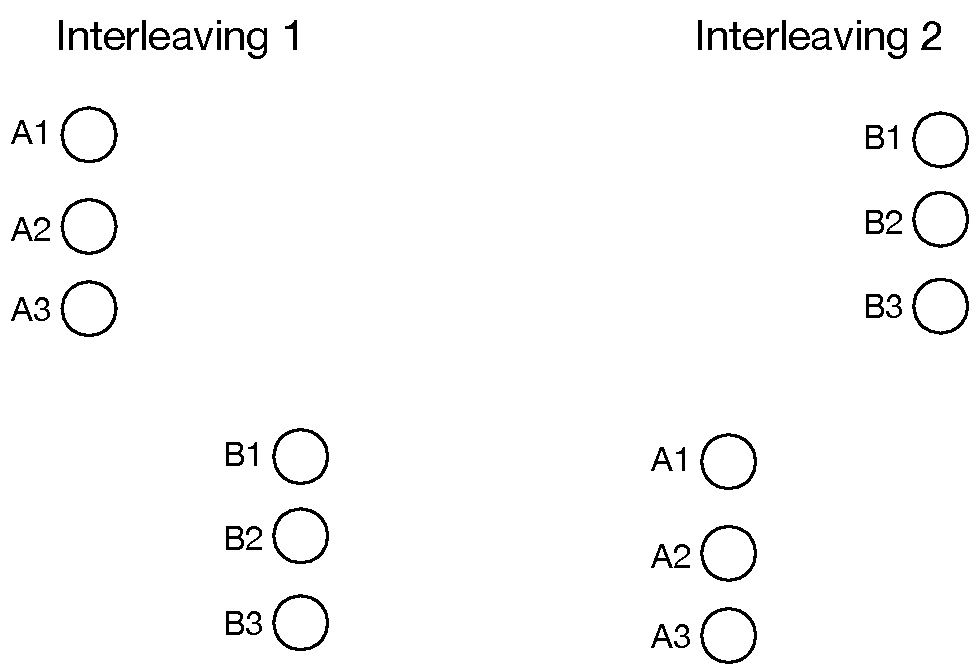
\includegraphics[width=0.95\linewidth]{fig/alias-coverage.pdf}
  \caption{Two instances of thread interleaving between thread~A and
    thread~B described in \autoref{fig:cve-2019-6974}. Regarding
    \texttt{inet->hdrincl}, alias coverage is saturated but the
    concurrency bug doest not manifest.}
  \label{fig:alias-coverage}
\end{figure}

\dr{say: existing coverage metrics either are coarse-grained (e.g.,
  Conzzer) or consider only a part of scheduling constraints (e.g.,
  KRace).}


\PP{Ineffective scheduling mechanism}

\dr{say: redundanct iterations of Razzer and Snowboard}

% In the perspective of fuzzing, a coverage metric is a paramount gear
% to determine whether a given input is worthy of further mutation.
% %
% If a coverage metric does not represent whether an input has a
% potential to trigger a race condition, a fuzzer may ignore inputs in
% which there are unexplored interleavings, or waste the computing power
% to valueless inputs.
% %
% In this regard, our primary question is whether existing coverage
% metrics in the concurrency dimension are suitable to apprehend
% interleavings potentially causing a race condition, for example,
% $(\texttt{A1} \rightarrow \texttt{B1}) \wedge (\texttt{B4} \rightarrow
% \texttt{A2})$ in \autoref{fig:cve-2019-6974}.



% Unfortunately, we observe that none of existing approaches incorporate
% a proper coverage metric for race conditions.
% %
% A few of existing approaches~\cite{snowboard, razzer} do not adopt a
% coverage in the concurrency dimension at all. Therefore, they do not
% make a decision as to whether a given input is worth further testing.
% %
% Other approaches~\cite{krace, muzz} adopt coverage metrics that are
% not suitable for race conditions as they do not consider a combined
% result of multiple pairs of conflicting accesses. As a consequence,
% race conditions may not be exposed even after the coverages are
% saturated.
% %
% % Consequently, existing approaches have difficulty in distinguishing a
% % given input has a potential to cause an interesting behavior, \ie,
% % a race condition.


% \begin{figure}[t]
%   \centering
%   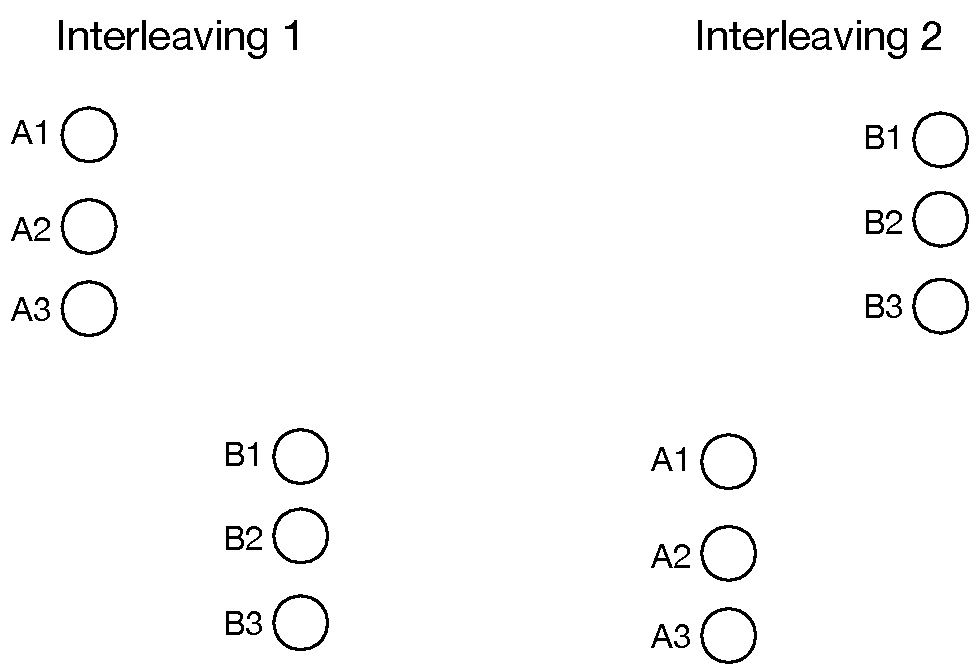
\includegraphics[width=0.98\linewidth]{fig/alias-coverage.pdf}
%   \caption{Three inputs that consist of two concurrent syscalls. For
%     all inputs, thread~A executes the same \texttt{mmap()} syscall
%     while thread~B handles different ioctl requests. For brevity, we
%     describe only conflicting instructions.\dr{Change the name of two
%       ioctls in input 1 and 2}}
%   \label{fig:alias-coverage}
% \end{figure}

% \yj{This is the key paragraph to point out the limitation of previous approaches, but very vague. Make specific claims of why Kraces' alias coverage is insufficient by giving an example.}
% %
% In order to show why comprehending multiple pairs of conflicting
% accesses is important, let us suppose we have three inputs that
% consists of two concurrent syscalls as described in
% \autoref{fig:alias-coverage}.
% %
% For all inputs, thread~A executes a \texttt{mmap()} syscall to map the
% binder driver to a user address space while thread~B handles different
% ioctl requests such that \texttt{ioctl(FREE_BUFFER)},
% \texttt{ioctl(REPLY)}, and \texttt{ioctl(TRANSACTION)} for
% \texttt{Input 1}, \texttt{Input 2}, and \texttt{Input 3} respectively.
% %
% It is worth noting that in \texttt{Input 1} and \texttt{Input 2},
% there is only one pair of conflicting accesses; in \texttt{Input 1},
% the two threads conflict on \texttt{alloc->vma}, and in \texttt{Input
%   2}, the two threads conflict on \texttt{alloc->mm}.



% \begin{figure}[t]
%   \centering
%   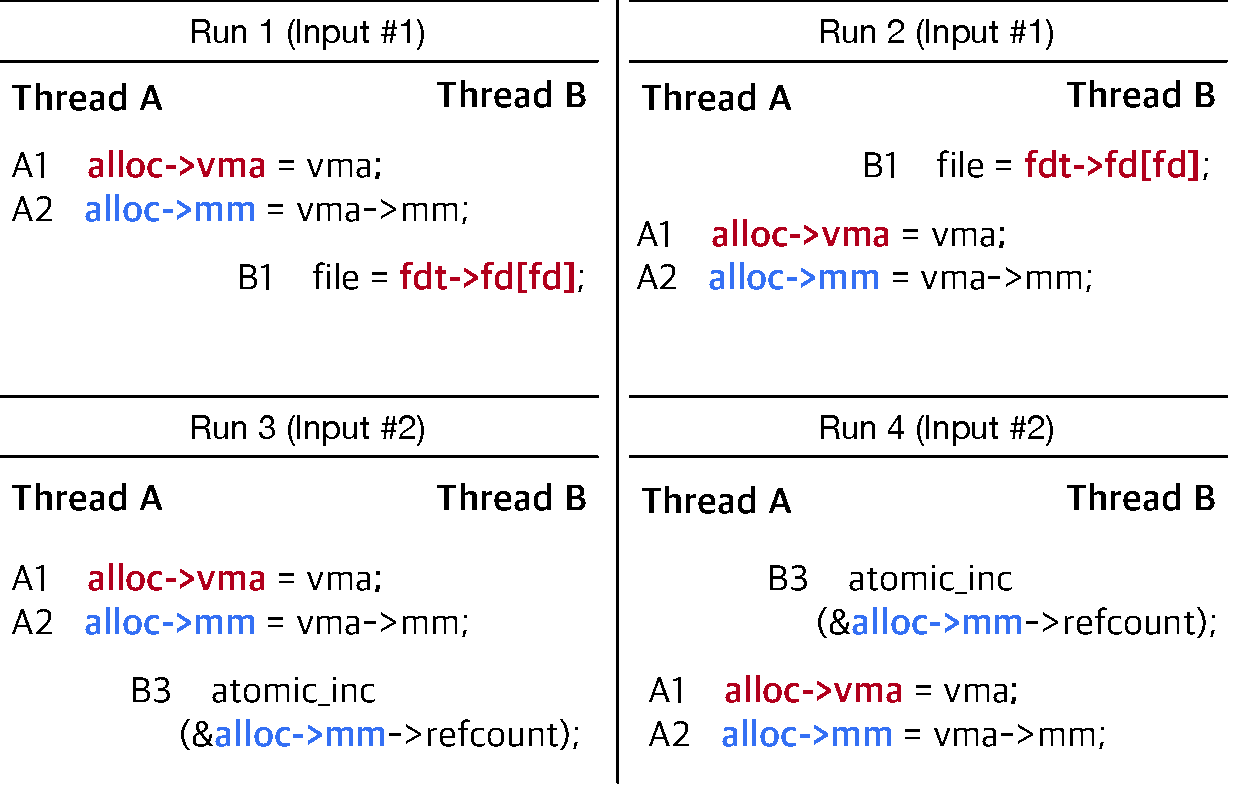
\includegraphics[width=0.9\linewidth]{fig/alias-coverage-interleaving.pdf}
%   \caption{Four interleavings of \texttt{Input 1} and \texttt{Input 2}
%     in \autoref{fig:alias-coverage}. After executing these four
%     interleavings, all possible execution orders of a single
%     conflicting accesses are exhibited.\dr{Run 1 -> Interleaving 1?}}
%   \label{fig:alias-coverage-interleaving}
% \end{figure}

% In this example, if we adopt a coverage metric that focuses on a
% single pair of conflicting accesses (\eg, alias coverage), a fuzzer
% may not recognize that \texttt{Input 3} may exhibit a different
% behavior than \texttt{Input 1} and \texttt{Input 2}~(\ie, a
% NULL-dereference bug).
% %
% \autoref{fig:alias-coverage-interleaving} shows four interleavings
% that exhibits all execution order of a single pair of conflicting
% accesses. If a fuzzer executes \texttt{Input 1} with interleavings in
% \texttt{Run 1} and \texttt{Run 2}, a fuzzer observes execution orders
% such as $\texttt{A1} \rightarrow \texttt{B1}$ (in \texttt{Run 1}) and
% $\texttt{B1} \rightarrow \texttt{A1}$ (in \texttt{Run 2}).
% %
% Similary, if a fuzzer executes \texttt{Input 2} with interleavings in
% \texttt{Run 3} and \texttt{Run 4}, it observes execution orders of
% $\texttt{A2} \rightarrow \texttt{B4}$ (in \texttt{Run 3}) and
% $\texttt{B4} \rightarrow \texttt{A2}$ (in \texttt{Run 4}).
% %
% After executing these four interleavings, \texttt{Input 3} does not
% reveal a new execution order of a single conflicting
% accesses. Therfore, as a Krace state, a fuzzer may de-prioritize
% \texttt{Input 3}, and the race condition may not be found.

% In summary, in order to determine whether an input shows interesting
% behaviors or not, a fuzzer needs to comprehend \textit{a combined
%   result of multiple pairs of conflicting accesses} as it is the
% primary reason of race conditions.



%%% Local Variables:
%%% mode: latex
%%% TeX-master: "p"
%%% End:
